The first step in the process of reconstructing the 3D geometry of the object is to establish a mathematical relationship between the natural units of the camera with the physical units of the 3D world. We used camera calibration to learn the internal parameters of the camera and its distortion coefficients. The geometry is described in terms of camera's optical center and focal length.

\begin{figure}[ht!]
\centering
\subfigure{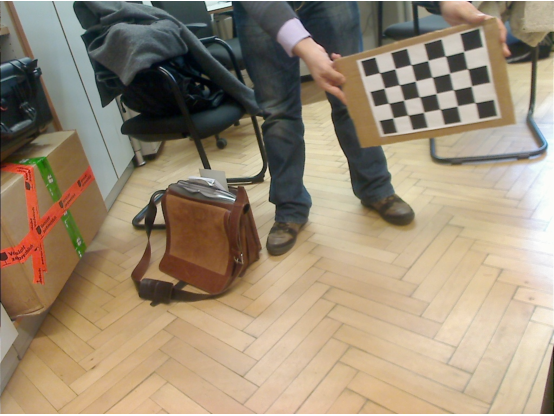
\includegraphics[width=.45\linewidth]{figures/calibrate-1}}\quad
\subfigure{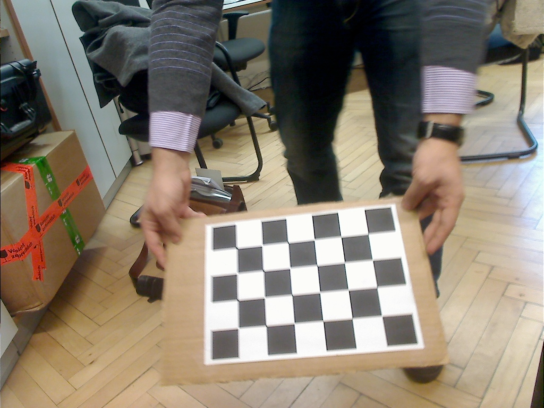
\includegraphics[width=.45\linewidth]{figures/calibrate-2}} \\
\subfigure{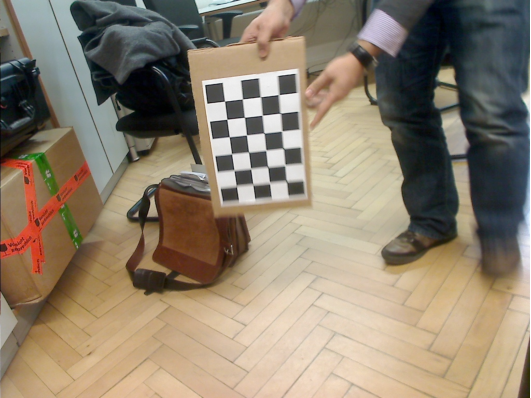
\includegraphics[width=.45\linewidth]{figures/calibrate-3}}\quad
\subfigure{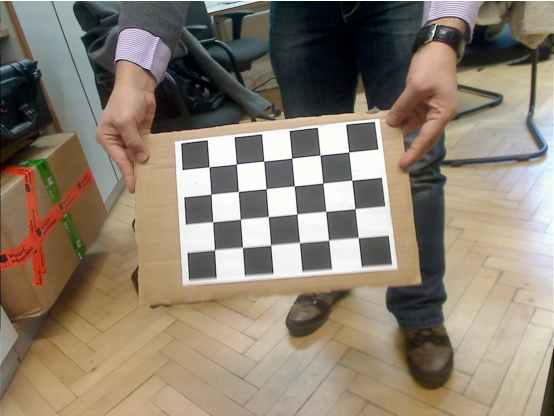
\includegraphics[width=.45\linewidth]{figures/calibrate-4}}
\caption{Calculating the Camera's Intrinsic Parameters}
\label{figure:camera-calibration-intrinsics}
\end{figure}

We used OpenCV routines that are based on \cite{zhang:2000} \cite{brown:1971} and used a planar chessboard pattern as our calibration object. We rotated and translated the pattern to provide multiple views to get the precise information about the intrinsic parameters of the camera as shown in figure \ref{figure:camera-calibration-intrinsics}. 
We used OpenCV routine \texttt{cvFindChessboardCorners()} to locate the corners and once we had enough corners from multiple view images, we used \texttt{cvCalibrateCamera2()} to get the intrinsic matrix $A$ as shown in equation \ref{equation:calibrate}.


\begin{align}
	\label{equation:calibrate}				
	s \times 
	\begin{bmatrix}
		u \\ v \\	1 \\
	\end{bmatrix} &= A \times \begin{bmatrix}
															R \mid T
	 				  								\end{bmatrix} 
										 \times \begin{bmatrix}
															x_w \\ y_w \\ z_w \\ 1
														\end{bmatrix} \\
	\text{where}~	 
	A &= \begin{bmatrix}
					f_x & 0 & c_x \\
					0 & f_y & c_y \\
					0 & 0 & 1 \\										
 		 	 \end{bmatrix} \notag
\end{align}

The intrinsic matrix $A$ was later used to describe the \emph{pose} of the objects being scanned by the laser relative to the coordinate system of the camera. In order to determine this pose on both sides of the target object, the patterns were masked out to allow individual calculation as shown in figure \ref{figure:camera-calibration-extrinsics}. The parameters represented by $\begin{bmatrix}R \mid T\end{bmatrix}$ could then be separately calculated for both the sides by calling the OpenCV routine \texttt{cvFindExtrinsicCameraParams2()}. 

\begin{figure}[ht!]
\centering
\subfigure[$R_1 \mid T_1$]
{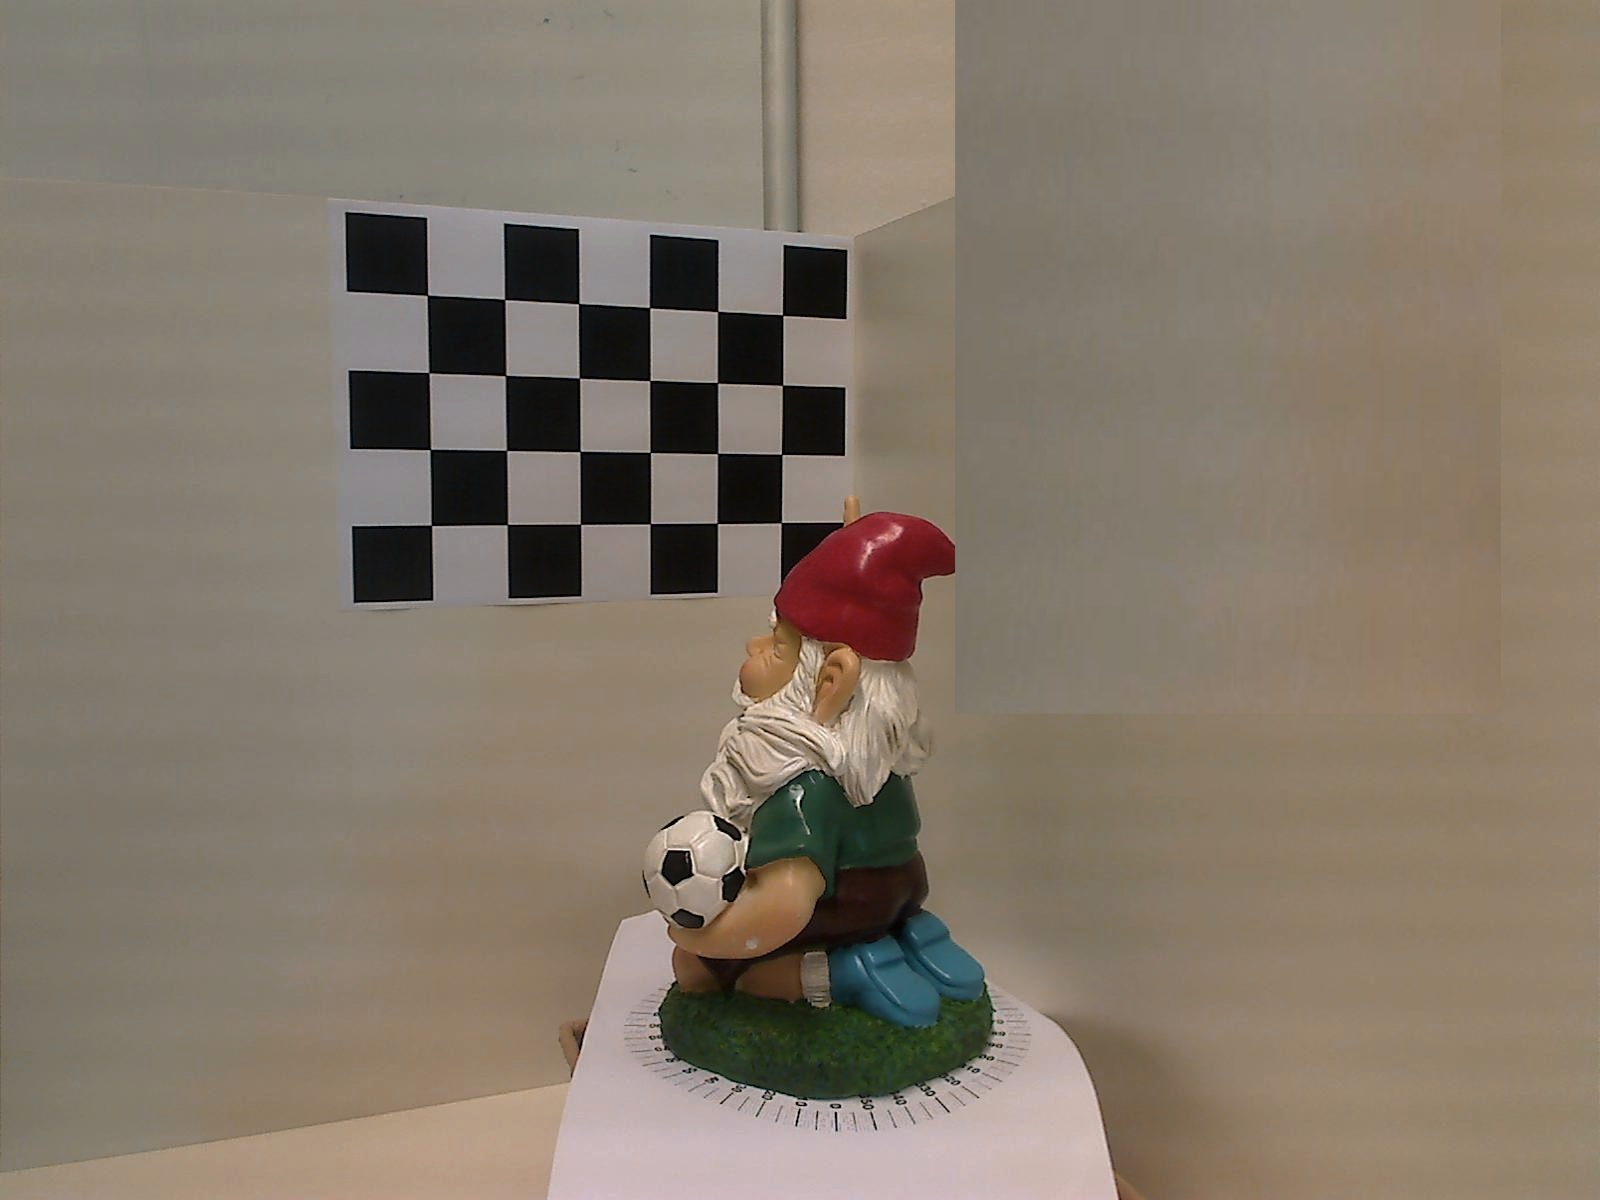
\includegraphics[width=.45\linewidth]{figures/calibrate-5}} \quad
\subfigure[$R_2 \mid T_2$]
{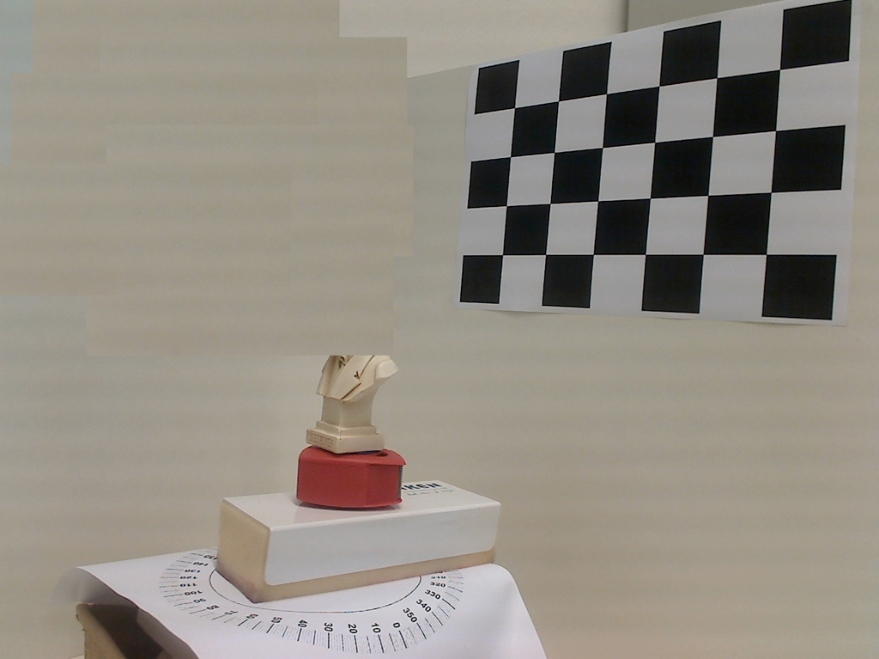
\includegraphics[width=.45\linewidth]{figures/calibrate-6}}
\caption{Calculating the Camera's Extrinsic Parameters}
\label{figure:camera-calibration-extrinsics}
\end{figure}